% !TEX root = 0_main.tex
\subsection*{Teilaufgabe 1: Theoretische Informatik} % TI
\begin{aufgabe}%1
\begin{teile}
	\item
\end{teile}	
\end{aufgabe}

\begin{aufgabe}%2
\begin{teile}
	\item
\end{teile}	
\end{aufgabe}


\begin{aufgabe}%3
\begin{teile}
	\item
\end{teile}	
\end{aufgabe}


\begin{aufgabe}%4
\begin{teile}
	\item
\end{teile}
\end{aufgabe}	

\begin{aufgabe}%5
\end{aufgabe}

\newpage
\subsection*{Teilaufgabe 2: Algorithmen} % A&D

\newcommand{\code}[1]{{\larger\texttt{#1}}}

\setcounter{aufgcount}{0}

\begin{aufgabe}%1
Bereits gelöst.
\end{aufgabe}


\begin{aufgabe}%1
\begin{teile}	
	\item
	Um das Minimum von \code{n} Zahlen zu ermitteln, müssen (in einer unsortierten Datenstruktur) alle Zahlen betrachtet werden. Ein Vergleich findet immer zwischen zwei Zahlen statt: dem aktuellen Minimum und der noch nicht betrachteten. 
	
	Das erfordert \code{n-1} Vergleiche. \\
	
	\item
	\begin{java}
	public static int maximum(int[] r) {
	    int max = r[0];
	    for (int i = 1; i < r.length; i++)
	        if (r[i] > max) 
	            max = r[i]; 
	    return max;
	}
	\end{java}
	
	Und hier noch in Pseudocode, wenn es unbedingt sein muss:
	\begin{java}
	Funktion maximum(r: Ganzzahlreihung) -> Ganzzahl {
       max = r[0]
       fuer i von 1 bis n-1
           wenn r[i] > max
               max = r[i]
       gib max zurueck
   }   
	\end{java}
	
	\newpage
	\item
	Pseudocode ist hier nicht ausdrücklich gefordert, also sparen wir ihn uns: 
	\begin{java}
	public static int[] maximumUndMinimum(int[] r) {
	    int[] minUndMax = new int[2];
	    int max, min;
	    min = max = r[0];
	    for (int i = 1; i < r.length; i++) {
	        if      (r[i] > max) max = r[i]; 
	        else if (r[i] < min) min = r[i];
	    }
	    minUndMax[0] = min;
	    minUndMax[1] = max;
	    return minUndMax;
	}
	\end{java} 
	
	Der \code{else}-Fall in der \code{for}-Schleife, der zuständig ist für die Aktualisierung des Minimums, wird nur dann betrachtet, wenn wir bereits wissen, dass das betrachetete Element nicht größer ist als das aktuelle Maximum.
	 
	Die Minimum-Vergleiche werden also nur dann angestellt, wenn wir das aktuelle Prüfelement bereits ausgeschlossen haben als Kandidat für das Maximum.
	
	So benötigen wir nur einen Durchlauf mit deutlich weniger Vergleichen. 
	
	
\end{teile}
\end{aufgabe}

\newpage
\begin{aufgabe}
\begin{teile}
	\item
	Ein schwach zusammenhängender Graph $G_n$ mit $n$ Knoten, bei dem O(n) Breitensuchen gestartet werden müssen, gestaltet sich sternförmig, wobei die Zacken des Sterns Knoten enthalten, die eine ausgehende Kante haben, die auf den mittleren Knoten gerichtet ist. 

	Damit muss von jedem Zacken-Knoten eine eigene Breitensuche gestartet werden. Beim ersten mal wird dann der Zacken und die Mitte besucht, anschließend bloß nur noch der jeweilige Zacken. Im Schlimmstfall beginnt die erste Breitensuche auch noch in der Mitte, dann sind genau $n$ Breitensuchen vonnöten, andernfalls $n-1$.

	Ein Beispielgraph mit 9 Knoten sähe dann so aus: 

\begin{center}
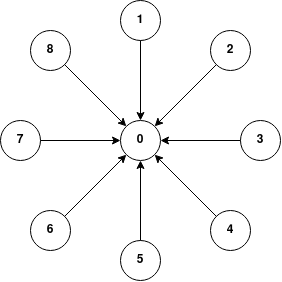
\includegraphics[scale=0.7]{Graph}
\end{center}

	\item
	Die Laufzeit beträgt O(n), denn es müssen O(n) Breitensuchen gestartet werden, wobei jede einzelne Breitensuche in O(1) abläuft, da sie jeweils nur höchstens einen Nachbarknoten besucht. 	
	
\end{teile}
\end{aufgabe}

\newpage
\begin{aufgabe}
\begin{teile}
	\item
	Dieser Graph \code{G} ermittelt für Dijkstra und Prim unterschiedliche Spannbäume:
	
	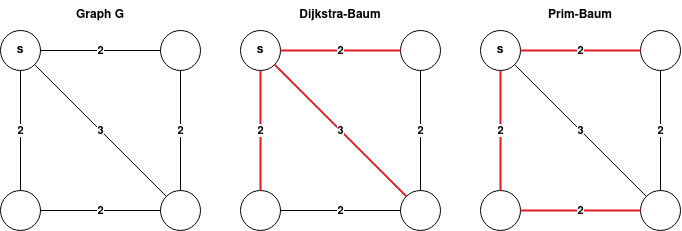
\includegraphics[scale=0.6]{Dijkstra_a} \\

	\item
	Bei Prim hängt die Laufzeit stärker ab von der Anzahl der Knoten, bei Kruskal stärker von der Anzahl der Kanten. Also schneidet Kruskal bei stark verzweigten Graphen schlechter ab als Prim. 
	
	Die maximale Anzahl an Kanten in einem (so genannten \glqq vollständigen\grqq) Graphen (bei dem jeder Knoten verbunden ist mit jedem anderen Knoten) beträgt: $m = \frac{n \cdot (n - 1)}{2}$
	
	Für große $n$ geht $m$ also gegen $n^2$. Damit gilt:
	
	$\overbrace{n^2 + n \cdot log(n)}^{Prim} < 
	\overbrace{n^2 \cdot log (n^2)}^{Kruskal}$ 
	
	Bereits für $n = 5$ ist diese Ungleichung erfüllt. Die Menge kann man also definieren als die Menge aller vollständigen Graphen mit $n \geq 5$.\\
	
	\item
	Für einen zusammenhängenden Graph $G$ mit $n$ Knoten gilt: $n - 1 \leq m \leq \frac{n \cdot (n - 1)}{2}$
	 
	Bei minimaler Kantenanzahl würde also gelten: $log (n-1) \in \theta(log(n))$
	
	Für $m > n$ würde allerdings gelten: $log(m) \notin \theta(log(n))$
	
	Also gilt $log (m) \in \theta(log(n))$ nur dann, wenn $m \leq n$.
	 
	
	
\end{teile}
\end{aufgabe}

\newpage
\begin{aufgabe}
\begin{teile}
	\item
	Das Problem kann modelliert werden mit einem gerichteten azyklischen Graph mit gewichteten Kanten, wobei jeder Knoten des Graphen eine Aufgabe darstellt und eine gerichtete Kanten die Erledigungsreihenfolge der Aufgaben darstellen, und die Kantengewichte die Erledigungsdauer.

	Laut Anforderung gibt es für jede Aufgabe \code{a} eine Menge von Nachfolgern \code{N(a)}, die die Aufgaben enthält, die erst erledigt werden können, nachdem \code{a} abgeschlossen ist. Modelliert wird dies durch die Richtung der Kanten, so dass der Knoten der Aufgabe \code{a} ausgehende Kanten hat, die gerichtet sind auf die Nachfolger aus \code{N(a)}.

	Analog werden Vorgänger eines Knotens  \code{a} modelliert als Knoten, die eine Kante haben, die gerichtet ist auf \code{a}. Hat Knoten \code{b} eine Kante, die gerichtet ist auf Aufgabe \code{a}, ist \code{b} also ein Vorgänger von \code{a}, und muss erst erledigt werden, bevor begonnen werden kann mit \code{a}.
	
	Schließlich gibt das Gewicht \code{w(a,b)} einer Kante von \code{a} nach \code{b} an, wie lange es dauert, bis Aufgabe \code{a} erledigt ist, was (mit den anderen Vorgängeraufgaben von \code{b}) eine Voraussetzung dafür ist, dass begonnen werden kann mit der Erledigung von \code{b}. \\
	
	\item
	Das hängt davon ab, dass der Graph eine Baumstruktur aufweist, wobei die Kindknoten eines jeden Knotens die Vorgänger darstellen.
	
	Eine Baumstruktur ist ja letztlich ein gerichteter azyklischer Graph, wie wir ihn oben modelliert haben, mit der Besonderheit, dass er keine Kreisläufe enthält. \\
	In einer Baumstruktur gibt es genau einen Pfad von jedem Knoten zum Wurzelknoten, und es gibt keine Abhängigkeiten zwischen den Knoten, die nicht entlang dieses Pfades verlaufen.
	
	Wenn die Aufgaben des Projekts so organisiert sind, dass sie eine Baumstruktur bilden, in der die Abhängigkeiten nur zwischen dem Vorgänger- und Nachfolgerknoten bestehen, dann können sie abgearbeitet werden in der Reihenfolge des Baumpfades bzw. der Ebenen des Baumes. \\
	
	\item
	Die Reihenfolge ergibt sich hier aus der Tiefe der jeweiligen Knoten innerhalb des Baumes. Je tiefer ein Knoten im Baum gelegen ist, desto früher wird er abgearbeitet in der Reihenfolge, zuerst also die Blattknoten der untersten Ebene.
	
	Um einen Projektplan mit Aufgaben in der entsprechenden Reihenfolge zu berechnen, muss der Graph traversiert werden in \textit{Reverse-Level-Order}, auf Gutdeutsch also mit einer \textit{umgekehrten Breitensuche}.
	 
	Bei der Breitensuche wird der Baum schichtenartig traversiert, es werden also alle Knoten der Baumebene hinzugefügt in den Aufgabenstapel, bevor die nächsttiefere Ebene betreten wird. Hier benötigen wir also die umgekehrte Variante, so dass bei der allerletzten Ebene begonnen und der Graph aufwärts weiterverarbeitet wird. 
	
	Die umgekehrte Breitensuche liefert uns somit den vollständigen Projektplan. \\
	
	\item
	Die Dauer des Projektes ergibt sich aus der Summe der jeweils längsten Kanten aus allen Ebenen des Baumes.
	
	Eine jeweilige Aufgabe kann erst begonnen werden, wenn alle Vorgänger erledigt sind. Die Startzeit $s_i$ einer Aufgabe $a_i$ ergibt sich also aus dem maximalen Wert aus der Summe der Endzeiten $e_j$ aller Vorgänger $j$ aus $N(i)$ und der Zeitdauer $w(j,i)$ zwischen $j$ und $i$. 
	
	So wird modelliert, dass eine Aufgabe erst gestartet wird, wenn alle ihre Vorgänger abgeschlossen sind. Anschließend wird die Endzeit $e_i$ einer Aufgabe $a_i$ berechnet als die Summe aus der Startzeit $s_i$ und der Dauer $l(a_i)$ der Aufgabe. 
	
	Ein möglicher Algorithmus könnte also aussehen wie folgt:

	\begin{enumerate}
        \item Initialisiere $s_1 = 0$ und $e_1 = l(a_1)$.
        \item
        Für alle $i$ von 2 bis $n$:
        \begin{itemize}
        	\item Setze $s_i = max(e_j + w(j, i))$, wobei $j$ über alle Elemente in $N(i)$ läuft.
        	\item Setze $e_i = s_i + l(a_i)$.
    	\end{itemize}
    	\item Optional: Gib die Start- und Endzeiten $s_i$ und $e_i$ aus für alle $i$ von 1 bis $n$.
        \end{enumerate}
    
	Die Endzeit des Wurzelknotens steht damit gleichzeitig für die Gesamtdauer des Projekts.
	\end{teile}
	\end{aufgabe}
	
\newpage


\begin{aufgabe}
\begin{teile}
	\item
	Die Sondierfolge $s(k, i) = (h(k) + 2i)$ mod $m$ ist eine \textbf{lineare Sondierung}, bei der der Wert $2i$ zum Streuwert h(k) addiert wird. 
	
	Problematisch an dieser Sondierfolge ist, dass sie viele Kollisionen erzeugt. Das liegt daran, dass das Addieren von $2i$ zum ursprünglichen Streuwert bei jeder Iteration die Sondierfolge um eine gerade Anzahl von Schritten verschiebt. Werden zwei Schlüssel abgebildet auf den gleichen Streuwert, haben sie bei dieser Sondierfolge dieselbe Folge von Indizes. Sie würden also direkt hintereinander an denselben Positionen in der Tabelle eingefügt werden. 
	
	Das führt letztlich zu einer Verschlechterung der Such- und Einfügezeiten. \\
	
	
	\item
	Die Sondierfolge $s(k,i) = (h(k) + i(i+1))$ mod $m$ ist eine \textbf{quadratische Sondierung}, bei der das Quadrat von $i$ addiert wird. 
	
	Quadratisches Sondieren ist besser als lineares Sondieren, da es gleichmäßiger streut, und somit weniger Kollisionen erzeugt. 
	
	Das einzige Problem, was ich bei dieser Streufunktion sehe ist, dass für die Modulo-Zahl keine Primzahl verwendet wird. Dies würde nämlich zu einer noch gleichmäßigeren Streung führen. \\

	\item
	Die Sondierfolge $s(k, i) = (h(k) + i * h'(k))$ mod $m$ ist eine Form der \textbf{doppelten Streusondierung}, bei der eine zweite Streufunktion $h'(k)$ verwendet wird, um den Abstand zu berechnen zwischen den Sondierungspositionen. 
	
	Für jede der beiden Streufunktionen tritt eine Kollision auf mit einer Wahrscheinlichkeit von $\frac{1}{m}$. Hier sind $h$ und $h'$ unabhänglig, also tritt eine Kollision nur noch auf mit der Wahrscheinlichkeit von $\frac{1}{m^2}$. Durch das Addieren von $h'(k)$ kann also eine sehr gleichmäßige Streuung erzeugt werden. \\
	

	\item
	\newcolumntype{X}{>{\centering}p{0.02\textwidth}}
	\begin{tabular}[t]{r|X|X|X|X|X|X|c}
	\textbf{Index} & 0 & 1 & 2 & 3 & 4 & 5 & 6 \\
	\hline
	\textbf{Eingefügter Schlüssel} & 2 & & 14 & 9 & & 3 & 8 \\
	\hline
	\textbf{Erfolglose Sondierungen} & & 8 \\ $\vert$ \\ 3 \\ $\vert$ \\ 2 & 3 \\ $\vert$ \\ 2 &  &  & 3 \\ $\vert$ \\ 2 
	\end{tabular}
	
	
	
\end{teile}
\end{aufgabe}

